%%
%% LaTeX template for UZH presentations.
%% (Riccardo Murri, <riccardo.murri@uzh.ch>)
%% 
%% Requires the `beamer` document class,
%% available at http://latex-beamer.sf.net/
%%
%% Use UTF-8 text (backwards compatible to ASCII, but not to
%% ISO-8859-1 and ISO-8859-15) or change the
%% `\usepackage[utf8x]{inputenc}` line below.
%%

\documentclass {beamer}
\mode<presentation>
{
  % for theme/color selection, see: http://www.hartwork.org/beamer-theme-matrix/
  \usetheme{CambridgeUS}
  \usecolortheme{dolphin}
  
  % no navigation bar
  \setbeamertemplate{navigation symbols}{}

  \logo{
\includegraphics[scale=0.17]{uzh-logo}}
  % To get just the UniZH coat of arms, use the following line instead:
  %\logo{
\includegraphics[scale=0.25,viewport=0 0 159 159]{uzh-logo}}
}


\title[GRunDB]% will appear on the bottom line
{Three tools for high-throughput computing with GAMESS}
\author[R.\ Murri]
{Riccardo Murri \\ \texttt{<riccardo.murri@uzh.ch>}}
\institute[GC3, Univ. of Zurich]% will appear on the bottom line
{\href{http://www.gc3.uzh.ch/}{Grid Computing Competence Centre}, 
  \href{http://www.uzh.ch/}{University of Zurich}
  \\ \url{http://www.gc3.uzh.ch/}}
\date[May 5, 2011]% will appear on the bottom line
  {May 5, 2011}


%% If you just use ASCII characters, you can safely remove the
%% following two lines:
\usepackage{ucs}
\usepackage[utf8x]{inputenc}

\usepackage[english]{babel}
\usepackage{graphicx}
\usepackage{array}
\usepackage{color}
\usepackage{hyperref}

%% Use `\largeskip` to get a larger vertical white space between two
%% lines/paragraphs:
\newcommand{\largeskip}{\vspace{1em}}
\def\+{\largeskip}

\begin{document}

\subject{Talks}
% This is only inserted into the PDF information catalog. Can be left
% out. 

\begin{frame}
  \titlepage
\end{frame}

% turn logo off after page 1
\expandafter\global\logo{}

% \begin{frame}
%   \frametitle{Talk outline}
%   \tableofcontents
%   % You might wish to add the option [pausesections]
% \end{frame}


%% Consult the `beamer` class documentation to know what kind of LaTeX
%% commands may be used here.  The following is just an example

\section{Introduction}

\begin{frame}
  \frametitle{Three tools for high-throughput GAMESS}

  \begin{description}
  \item[GRunDB] Compute energy of a set of molecules.
  \item[GGamess] Run an arbitrary set of GAMESS \texttt{.INP} files in parallel.
  \item[gc3libs.template] Generate a set of files from a given template.
  \end{description}

  The purpose of this talk is to determine whether these can be of any
  use to you or GC3 should stop supporting them.
\end{frame}

\section{GRunDB}

\begin{frame}
  \frametitle{What is GRunDB then?}
  
  GRunDB is a tool to automate:
  \begin{itemize}
  \item running GAMESS on a data-bank (GMTKN24) of molecule geometries
  \item comparing computed stoichiometry results with known-good ones
  \end{itemize}
\end{frame}

\begin{frame}
  \frametitle{Functional high-level view}

  GRunDB is implemented as a Linux command-line tool on top of the
  \href{http://gc3pie.googlecode.com/}{GC3Libs/GC3Utils} toolkit.
  % GRunDB interoperates with the GC3Utils job control commands: jobs
  % can be inspected, cancelled, re-submitted outside of GRunDB.

  \+
  GRunDB takes as input:
  \begin{itemize}
  \item a set of molecules (a subset of an online data-bank: either
    the original GMTKN24 or its local copy at UZH)
  \item a GAMESS input file (except the \texttt{\$DATA} section)
  \end{itemize}
  It creates a GAMESS job for each molecule in the subset, plugging
  its geometry in the template input file.

  \+
  When all jobs are done:
  \begin{itemize}
  \item results are extracted from the output files
  \item a summary table compares computed energy with reference data
  \end{itemize}

\end{frame}


\begin{frame}
  \frametitle{Architecture}

  \begin{center}
    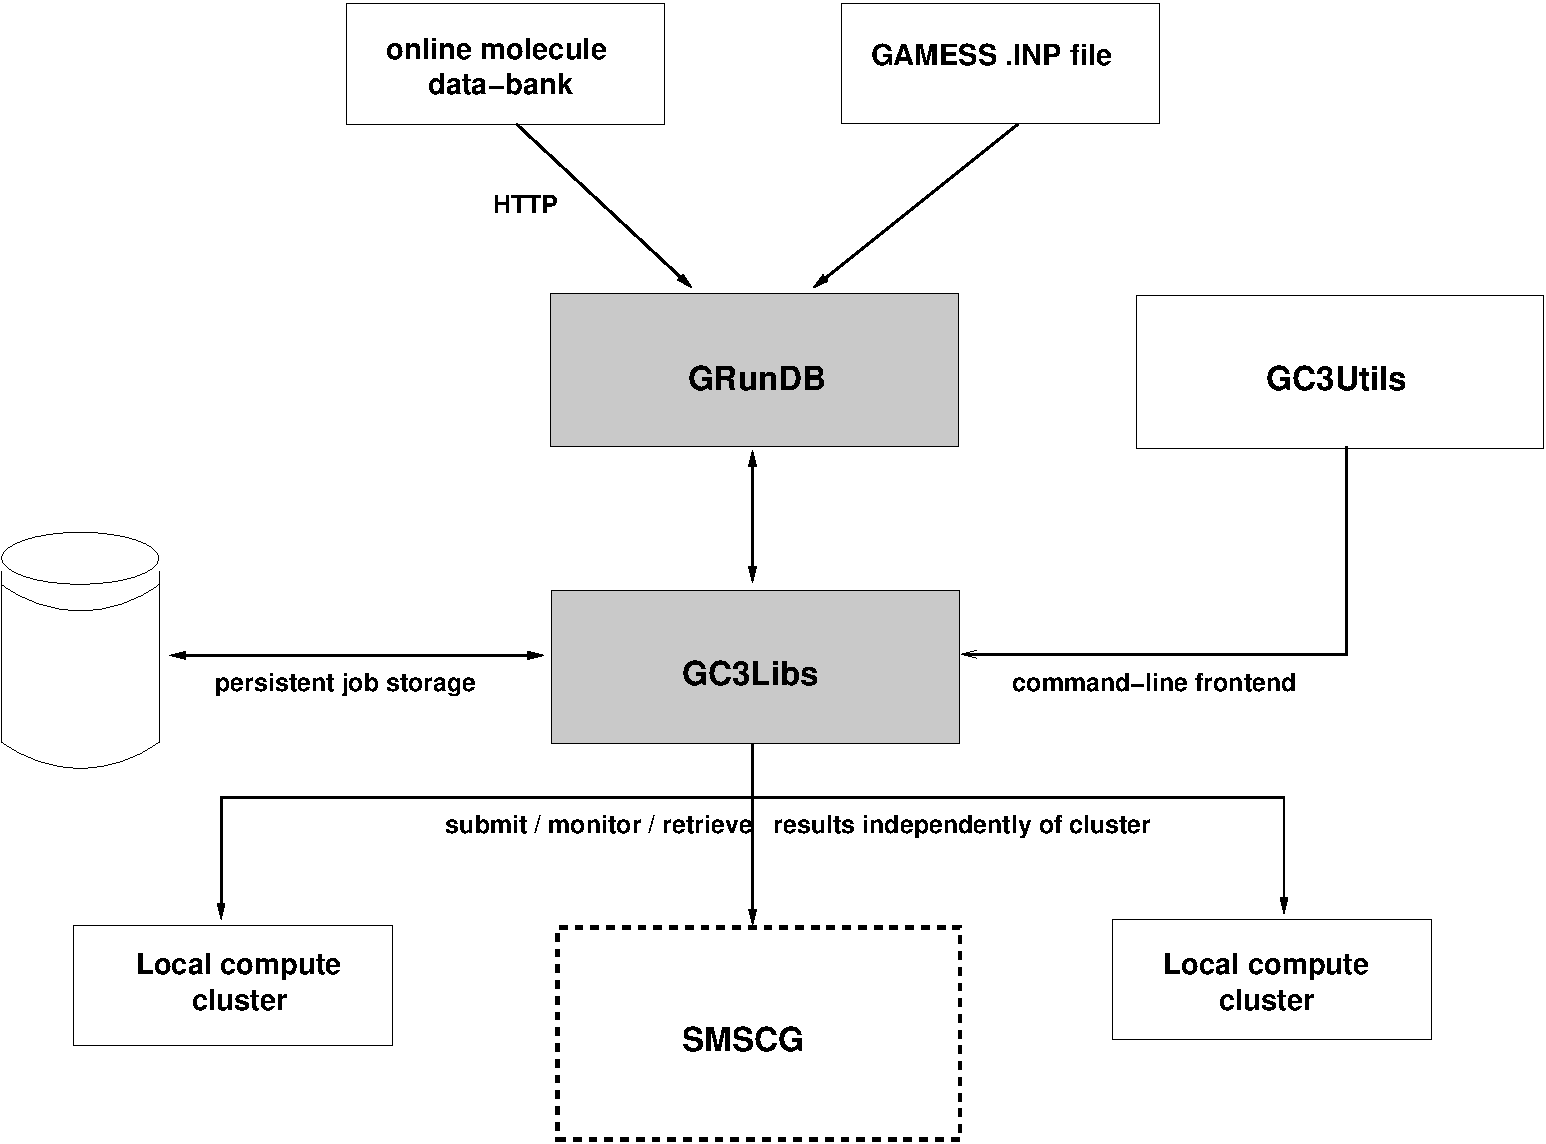
\includegraphics[width=0.8\textwidth]{architecture}
  \end{center}
\end{frame}

\begin{frame}
  \frametitle{The GAMESS.UZH molecule database: Subset index}
  \begin{center}
    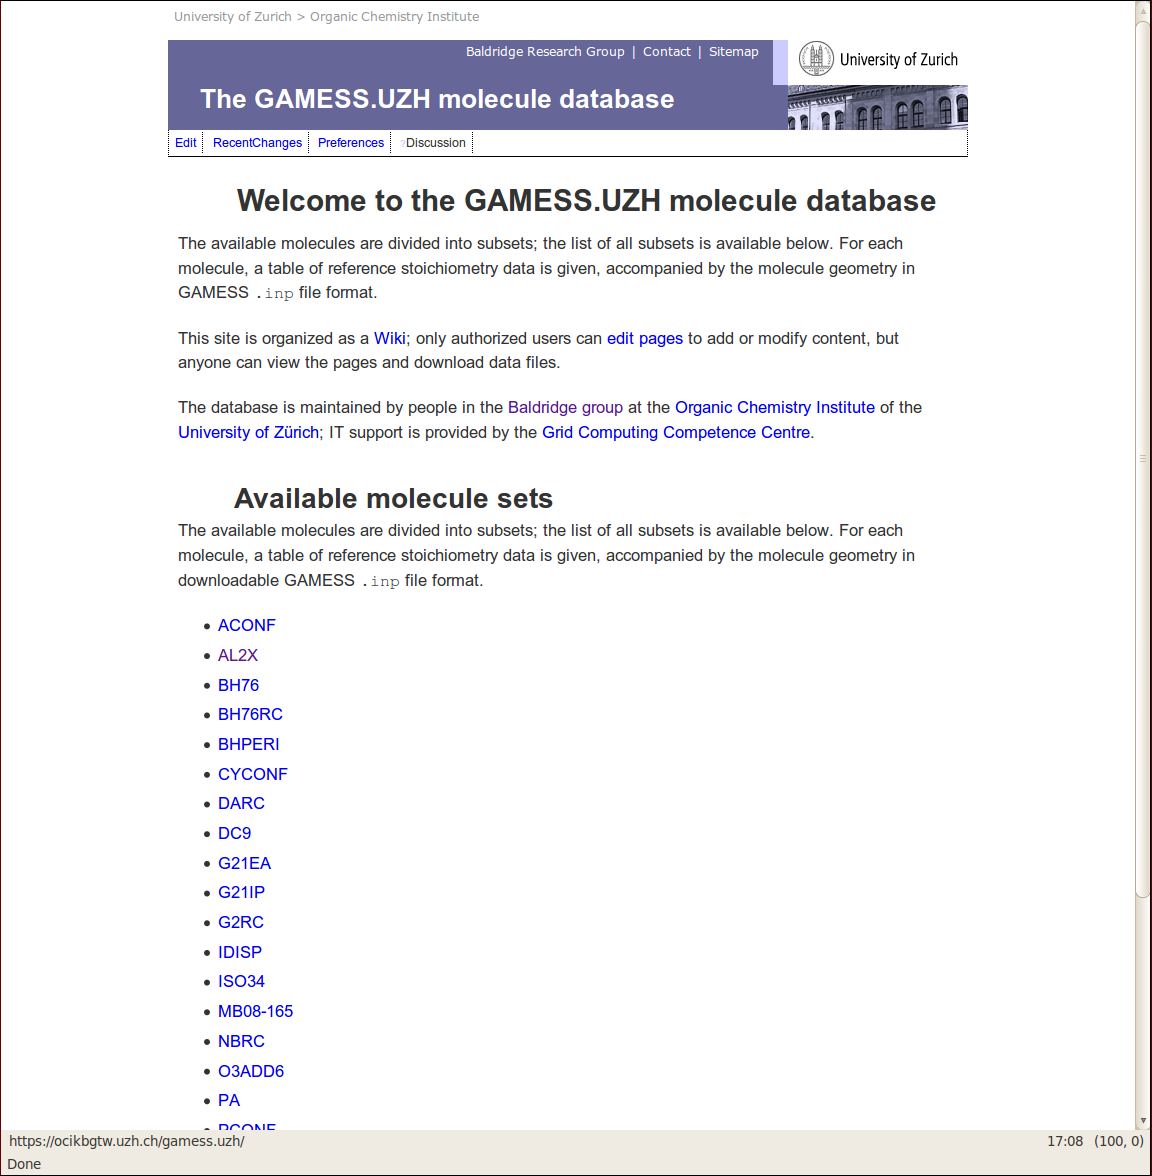
\includegraphics[height=0.9\textheight]{gamess-uzh-1}
  \end{center}
\end{frame}

\begin{frame}
  \frametitle{The GAMESS.UZH molecule database: The AL2X subset}
  \begin{center}
    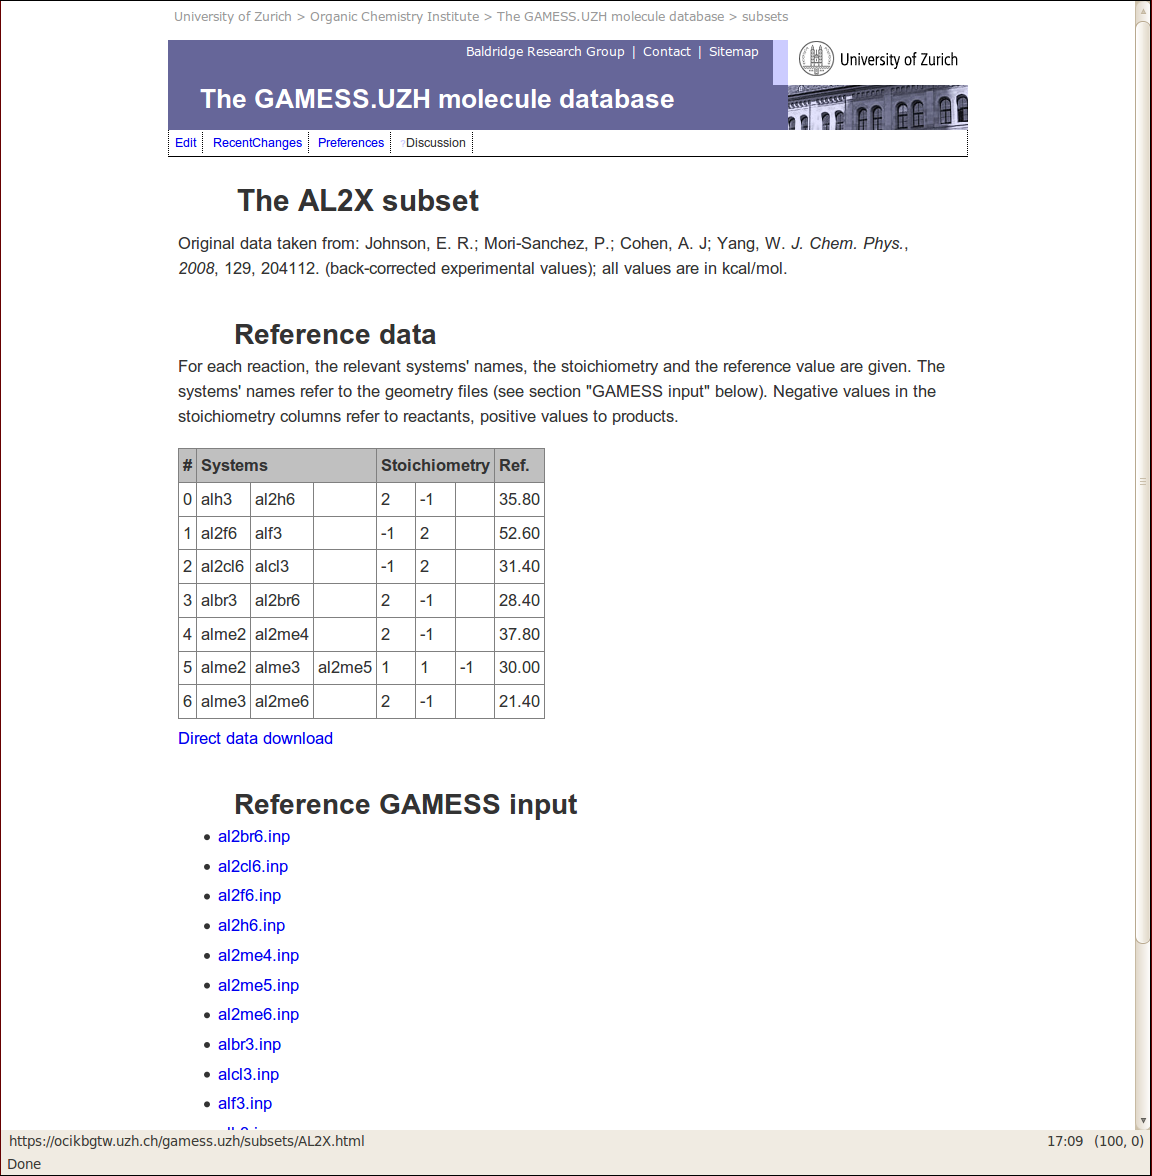
\includegraphics[height=0.9\textheight]{gamess-uzh-2}
  \end{center}
\end{frame}


\begin{frame}[fragile]
  \frametitle{Start analysis of a molecule set}

  GRunDB creates a job for each molecule in the specified subset.
  A \emph{session} name must be given to record the current analysis.

  \+ 
  Subsets can be specified by their name on the web page.  More
  than one (or \emph{ALL}) can be analyzed in a single GRunDB go.

  \+
  \begin{footnotesize}
\begin{semiverbatim}
\$ {\bf ./grundb.py new AL2X session1}
Input file name  State (JobID)       Info
==============================================================================
al2br6           NEW (job.680)       New at Mon Nov 29 14:06:46 2010
al2cl6           NEW (job.681)       New at Mon Nov 29 14:06:46 2010
al2f6            NEW (job.682)       New at Mon Nov 29 14:06:46 2010
al2h6            NEW (job.683)       New at Mon Nov 29 14:06:46 2010
{\em ...}
alf3             NEW (job.689)       New at Mon Nov 29 14:06:47 2010
alh3             NEW (job.690)       New at Mon Nov 29 14:06:47 2010
alme2            NEW (job.691)       New at Mon Nov 29 14:06:47 2010
alme3            NEW (job.692)       New at Mon Nov 29 14:06:47 2010
\end{semiverbatim}    
  \end{footnotesize}
\end{frame}

\begin{frame}[fragile]
  \frametitle{Submit jobs to the Grid}

  Once a session has been created, a single command invocation is
  needed to submit jobs to SMSCG or University clusters.
  \+
  \begin{footnotesize}
\begin{semiverbatim}
\$ {\bf ./grundb.py progress session1}
Insert AAI/Switch password for user  m1058036 :
Queue selected: all.q@idgc3grid01.uzh.ch
File uploaded: /tmp/rmurri/rsl.qOp5wn
File uploaded: /home/rmurri/gc3/gc3utils/0.10/grundb/take1.inp.d/AL2X/al2f6.inp
  {\em ...}
Input file name  State (JobID)       Info
==============================================================================
al2br6           SUBMITTED (job.680)  Submitted at Mon Nov 29 14:08:04 2010
al2cl6           SUBMITTED (job.681)  Submitted at Mon Nov 29 14:07:53 2010
al2f6            SUBMITTED (job.682)  Submitted at Mon Nov 29 14:07:29 2010
al2h6            SUBMITTED (job.683)  Submitted at Mon Nov 29 14:07:41 2010
  {\em ...}
alh3             SUBMITTED (job.690)  Submitted at Mon Nov 29 14:07:50 2010
alme2            SUBMITTED (job.691)  Submitted at Mon Nov 29 14:07:59 2010
alme3            SUBMITTED (job.692)  Submitted at Mon Nov 29 14:08:02 2010
\end{semiverbatim}    
  \end{footnotesize}
\end{frame}

\begin{frame}[fragile]
  \frametitle{Monitor job progress and execution}

  The same command is used to monitor job execution.
  \+
  \begin{footnotesize}
\begin{semiverbatim}
\$ {\bf ./grundb.py progress session1}
Input file name  State (JobID)       Info
==============================================================================
al2br6           SUBMITTED (job.680)  Submitted at Mon Nov 29 14:08:04 2010
al2cl6           RUNNING (job.681)   Running at Mon Nov 29 14:08:40 2010
al2f6            RUNNING (job.682)   Running at Mon Nov 29 14:08:40 2010
al2h6            RUNNING (job.683)   Running at Mon Nov 29 14:08:40 2010
  {\em ...}
alh3             RUNNING (job.690)   Running at Mon Nov 29 14:08:40 2010
alme2            SUBMITTED (job.691)  Submitted at Mon Nov 29 14:07:59 2010
alme3            SUBMITTED (job.692)  Submitted at Mon Nov 29 14:08:02 2010
\end{semiverbatim}    
  \end{footnotesize}
\end{frame}

\begin{frame}[fragile]
  \frametitle{Output retrieval and post-processing}

  Again, \texttt{grundb progress} will automatically retrieve and
  post-process results of jobs that have finished execution,
  extracting the energy values needed to compute stoichiometry results.
  \+
  \begin{footnotesize}
\begin{semiverbatim}
\$ {\bf ./grundb.py progress session1}
File downloaded: gsiftp://idgc3grid01.uzh.ch:2811/jobs/170571291036083905502916/alme3.out
File downloaded: gsiftp://idgc3grid01.uzh.ch:2811/jobs/170571291036083905502916/alme3.dat
  {\em ...}
Input file name  State (JobID)       Info
==============================================================================
al2br6           RUNNING (job.680)   Running at Mon Nov 29 14:09:00 2010
al2cl6           RUNNING (job.681)   Running at Mon Nov 29 14:08:40 2010
al2f6            DONE (job.682)      Final-b2plyp energy= -1084.1929109480 
al2h6            DONE (job.683)      Final-b2plyp energy= -488.2225951188 
  {\em ...}
alh3             DONE (job.690)      Final-b2plyp energy= -244.0835095562 
alme2            DONE (job.691)      Final-b2plyp energy= -322.6947308201 
alme3            DONE (job.692)      Final-b2plyp energy= -361.9996423212 
\end{semiverbatim}    
  \end{footnotesize}
\end{frame}

\begin{frame}[fragile]
  \frametitle{Finally...}

  When all jobs are done, GRunDB computes stoichiometry data and
  compares it to the reference data.

  \begin{scriptsize}
\begin{semiverbatim}
\$ {\bf ./grundb.py progress session1}
Input file name  State (JobID)       Info
==============================================================================
al2br6           DONE (job.682)      Final r-m06 energy is -15929.9575541891
  {\em ...}                                                     after 19 iterations 
alme3            DONE (job.694)      Final r-m06 energy is -362.1226427375
                                                           after 18 iterations 
STOICHIOMETRY DATA
Reaction                            Comp. energy  (Ref. data; deviation)
==============================================================================
                                     AL2X
------------------------------------------------------------------------------
2*alh3 + -1*al2h6                         +35.70  (+35.80; -0.10)
-1*al2f6 + 2*alf3                         +48.46  (+52.60; -4.14)
-1*al2cl6 + 2*alcl3                       +28.15  (+31.40; -3.25)
2*albr3 + -1*al2br6                       +25.41  (+28.40; -2.99)
2*alme2 + -1*al2me4                       +34.52  (+37.80; -3.28)
1*alme2 + 1*alme3 + -1*al2me5             +28.55  (+30.00; -1.45)
2*alme3 + -1*al2me6                       +21.72  (+21.40; +0.32)
\end{semiverbatim}    
  \end{scriptsize}
\end{frame}

\section{GGamess}

\begin{frame}
  \frametitle{What is GGamess then?}
  
  GGamess is a command-line tool to submit a set of GAMESS
  \texttt{.INP} files in parallel.
  \begin{itemize}
  \item For each job, manage the entire lifecycle: submit, monitor,
    retrieve output when done.
  \item Each job is independent of others.
  \item You can stop and restart it at a later time, processing
    continues from where it was interrupted.
  \item Finally exits when all jobs are done.
  \end{itemize}
\end{frame}

\begin{frame}[fragile]
  \frametitle{Example: running the GAMESS tests / 1}
  Running \texttt{ggamess} once submits the the jobs.

  \begin{scriptsize}
\begin{semiverbatim}
\$ \textbf{ls tests}
exam01.inp  exam02.inp  exam03.inp  exam04.inp  exam05.inp
\emph{[...]}
exam41.inp  exam42.inp  exam43.inp  exam44.inp 

\$ \textbf{./ggamess.py -r ocikbpra tests/}
Status of jobs in the 'ggamess' session: (at 11:14:23, 05/05/11)
        NEW   0/44     (0.0\%)
    STOPPED   0/44     (0.0\%)
  \textbf{SUBMITTED   44/44   (100.0\%)}
 TERMINATED   0/44     (0.0\%)
TERMINATING   0/44     (0.0\%)
      total   44/44   (100.0\%)
\end{semiverbatim}
  \end{scriptsize}
\end{frame}

\begin{frame}[fragile]
  \frametitle{Example: running the GAMESS tests / 2}
  Running it again updates status and fetches results of finished jobs.

  \+
  You can also request a detailed listing of the jobs with the
  \texttt{-l} option:
  \begin{scriptsize}
  \begin{semiverbatim}
\$ \textbf{./ggamess.py -l -r ocikbpra tests/}
 JobID     Job name     State                                    Info                               
===================================================================================================
job.8945   exam42     SUBMITTED    Submitted to 'smscg' at Thu May  5 11:11:58 2011                 
job.8944   exam16     SUBMITTED    Submitted to 'smscg' at Thu May  5 11:12:02 2011                 
\emph{[...]}
job.8937   exam20     TERMINATED   Execution of gamess terminated normally thu may  5 11:12:42 2011
job.8936   exam29     TERMINATED   Execution of gamess terminated normally thu may  5 11:12:43 2011
\end{semiverbatim}
  \end{scriptsize}

  Each job has its own output directory.
  \begin{scriptsize}
\begin{semiverbatim}
\$ \textbf{ls exam29}
exam29.dat  exam29.out
\end{semiverbatim}
  \end{scriptsize}
\end{frame}

\begin{frame}[fragile]
  \frametitle{Example: running the GAMESS tests / 3}

  Perhaps the most intersting thing is that you can tell
  \texttt{ggamess} to keep running until all jobs are done and their
  output retrieved.

  \+
  Example: keep running, and update job status every 20 seconds.
  \begin{scriptsize}
  \begin{semiverbatim}
\$ \textbf{./ggamess.py -r ocikbpra tests/ -C 20}
Status of jobs in the 'ggamess' session: (at 11:27:48, 05/05/11)
        NEW   0/44     (0.0\%)  
    STOPPED   0/44     (0.0\%)  
  SUBMITTED   5/44    (11.4\%)  
 TERMINATED   39/44   (88.6\%)  
TERMINATING   0/44     (0.0\%)  
         ok   39/44   (88.6\%)  
      total   44/44   (100.0\%) 
\emph{...continues running}
\end{semiverbatim}
  \end{scriptsize}
\end{frame}


\section{gc3libs.template}
\label{sec:templates}

\begin{frame}
  \frametitle{What is \texttt{gc3libs.template}?}

  \texttt{gc3libs.template} is a tool for generating a set of files
  from a template.

  \+
  It's a \emph{programming library}, not a command-line tool; you need
  to do some Python language programming to exploit it fully.
\end{frame}

\begin{frame}[fragile]
  \frametitle{Example: Timm's ``GAMESS benchmark'' / 1}

To use \texttt{gc3libs.template} you need:
\begin{enumerate}
\item A string with the template contents of the file;
\item actual parameters to be substituted in the template;
\item an optional ``filter function'' to determine which combination
  of parameters are acceptable.
\end{enumerate}

  \begin{scriptsize}
\begin{semiverbatim}
GAMESS_INP = Template("""
 \$\$CONTRL RUNTYP=ENERGY MAXIT=1 UNITS=BOHR \$\$END
 \$\$CONTRL \${SCF} ISPHER=\${ISPHER} \$\$END
 \$\$ACCURACY ITOL=\${ITOL} ILOAD=\${ILOAD} \$\$END
 \$\$SYSTEM MWORDS=10 \$\$END
 \$\$BASIS \${BASIS} \$\$END
 \$\$GUESS GUESS=HUCKEL \$\$END

 \$\$DATA
\${GEOMETRY}
 \$\$END
""",
   match_ispher_with_basis,
\end{semiverbatim}
  \end{scriptsize}
\end{frame}

\begin{frame}[fragile]
  \frametitle{Example: Timm's ``GAMESS benchmark'' / 2}

  Substitution parameters can be simple list of values (including
  multi-line strings).

  \begin{scriptsize}
\begin{semiverbatim}
GEOMETRY = [
        """Water
C1
O   8.0        0.0              0.0                    0.0
H   1.0        0.0              1.428036               1.0957706
H   1.0        0.0             -1.428036               1.0957706""",
        """Methane
Td

C     6.0   0.0            0.0            0.0
H     1.0   0.6252197764   0.6252197764   0.6252197764""",
        ],
\end{semiverbatim}
  \end{scriptsize}
\end{frame}

\begin{frame}[fragile]
  \frametitle{Example: Timm's ``GAMESS benchmark'' / 3}

  But they can be other templates, which are recursively expanded.
  \begin{scriptsize}
\begin{semiverbatim}
BASIS = [Template("GBASIS=\${SIMPLEBASIS}",
                  SIMPLEBASIS = ["MINI", "MIDI", "DZV", "TZV", 
                                 "CCD", "CCT", "CCQ", "CC5", "CC6"]),
         Template("GBASIS=\${GBASIS} NGAUSS=\${NGAUSS} \${NPFUNC} \${NDFUNC} \${NFFUNC}",
                  acceptable_gbasis_and_ngauss,
                  GBASIS = ["STO", "N21", "N31", "N311"],
                  NGAUSS = [2, 3, 4, 5, 6],
                  NPFUNC = ["", "NPFUNC=1"],
                  NDFUNC = ["", "NDFUNC=1"],
                  NFFUNC = ["", "NFFUNC=1"],
                  ),
         ],
\end{semiverbatim}
  \end{scriptsize}
\end{frame}

\section{This is the end...}
\label{sec:end}

\begin{frame}
  \begin{center}
    {\Huge Thank you!}
    \\
    \+
    {\Large (Any questions?)}
  \end{center}
\end{frame}

\begin{frame}
  \frametitle{Three tools for high-throughput GAMESS}

  \begin{description}
  \item[GRunDB] Compute energy of a set of molecules.
  \item[GGamess] Run an arbitrary set of GAMESS \texttt{.INP} files in parallel.
  \item[gc3libs.template] Generate a set of files from a given template.
  \end{description}
\end{frame}


\section{More information}

\begin{frame}
  \frametitle{Well, and the errors...?}

  Errors happen, and it's not necessarily a users' fault.  (e.g., disk
  full on a remote cluster)

  \+ How does GRunDB deal with this?

  \pause
  \+ Use GC3Utils to get control over the \emph{individual} job:
  \begin{itemize}
  \item Inspect job output and logs in the \emph{session.out.d}
    directory (or use the \texttt{gtail} command)
  \item Take measures against the failure
  \item Re-submit the failed job with \texttt{gresub}
  \item GRunDB will notice and re-process the results when the new job
    is done.    
  \end{itemize}

\end{frame}

\end{document}

%%% Local Variables: 
%%% mode: latex
%%% TeX-master: t
%%% x-symbol-8bits: nil
%%% End: 
